\documentclass[colorlinks=true,pdfstartview=FitV,linkcolor=blue,
            citecolor=magenta,urlcolor=red]{ligodoc}

\usepackage{graphicx}
\usepackage{hyperref}
\usepackage{amssymb}
\usepackage{amsmath}
\usepackage{longtable}
\usepackage{float}
\usepackage{rotating}
\usepackage[usenames,dvipsnames]{color}
\usepackage{fancyhdr}
\usepackage{subcaption}

%%%%%%%%%%%%%%%%%%%%%%%%%%%%%%
\title{Conditioning ring heater actuator input to optimize thermo-optic response}
\author{Daniel Vander-Hyde, Stefan Ballmer}
%\date{${}$Date: 2007/09/30}
\ligodccnumber{T}{19}{00496}{v0}{D} \ligodistribution{LIGO Scientific Collaboration}
%\ligodraft

%%%%%%%%%%%%%%%%%%%%%%%%%%%%%%%%%%%%%%%%%%%%%%%%%%%%%%%%%%%%%%%%%%%%%
\begin{document}

%%%%%%%%%%%%%%%%%%%%%%%%%%%%%%%%%%%%%%%%%%%%%%%%%%%%%%%%%%%%%%%%
\section{Overview}
\label{sec:I}
As the Advanced LIGO detectors reach $\approx$ 200kW of circulating power in the Fabry Perot arm cavities, ring heater actuation becomes cruicial for O3 comissioning but to achieve a required thermo-optic lens by adjusting the ring heater acutators it may take on the order of 10-12 hours (Fig \ref{fig:meas}) to reach a steady thermal lens. This results in a large amount of time the interferometer will be improperly mode matched and makes adjusting thermal compensation a laborious process. The thermo-optic step response of the LIGO test mass / ring heater system can be shortened to 2-4 hours with real time digital filtering of the ring heater actuator power input. The following sections describe the concept and design behind this filter.

\begin{figure}[H]
 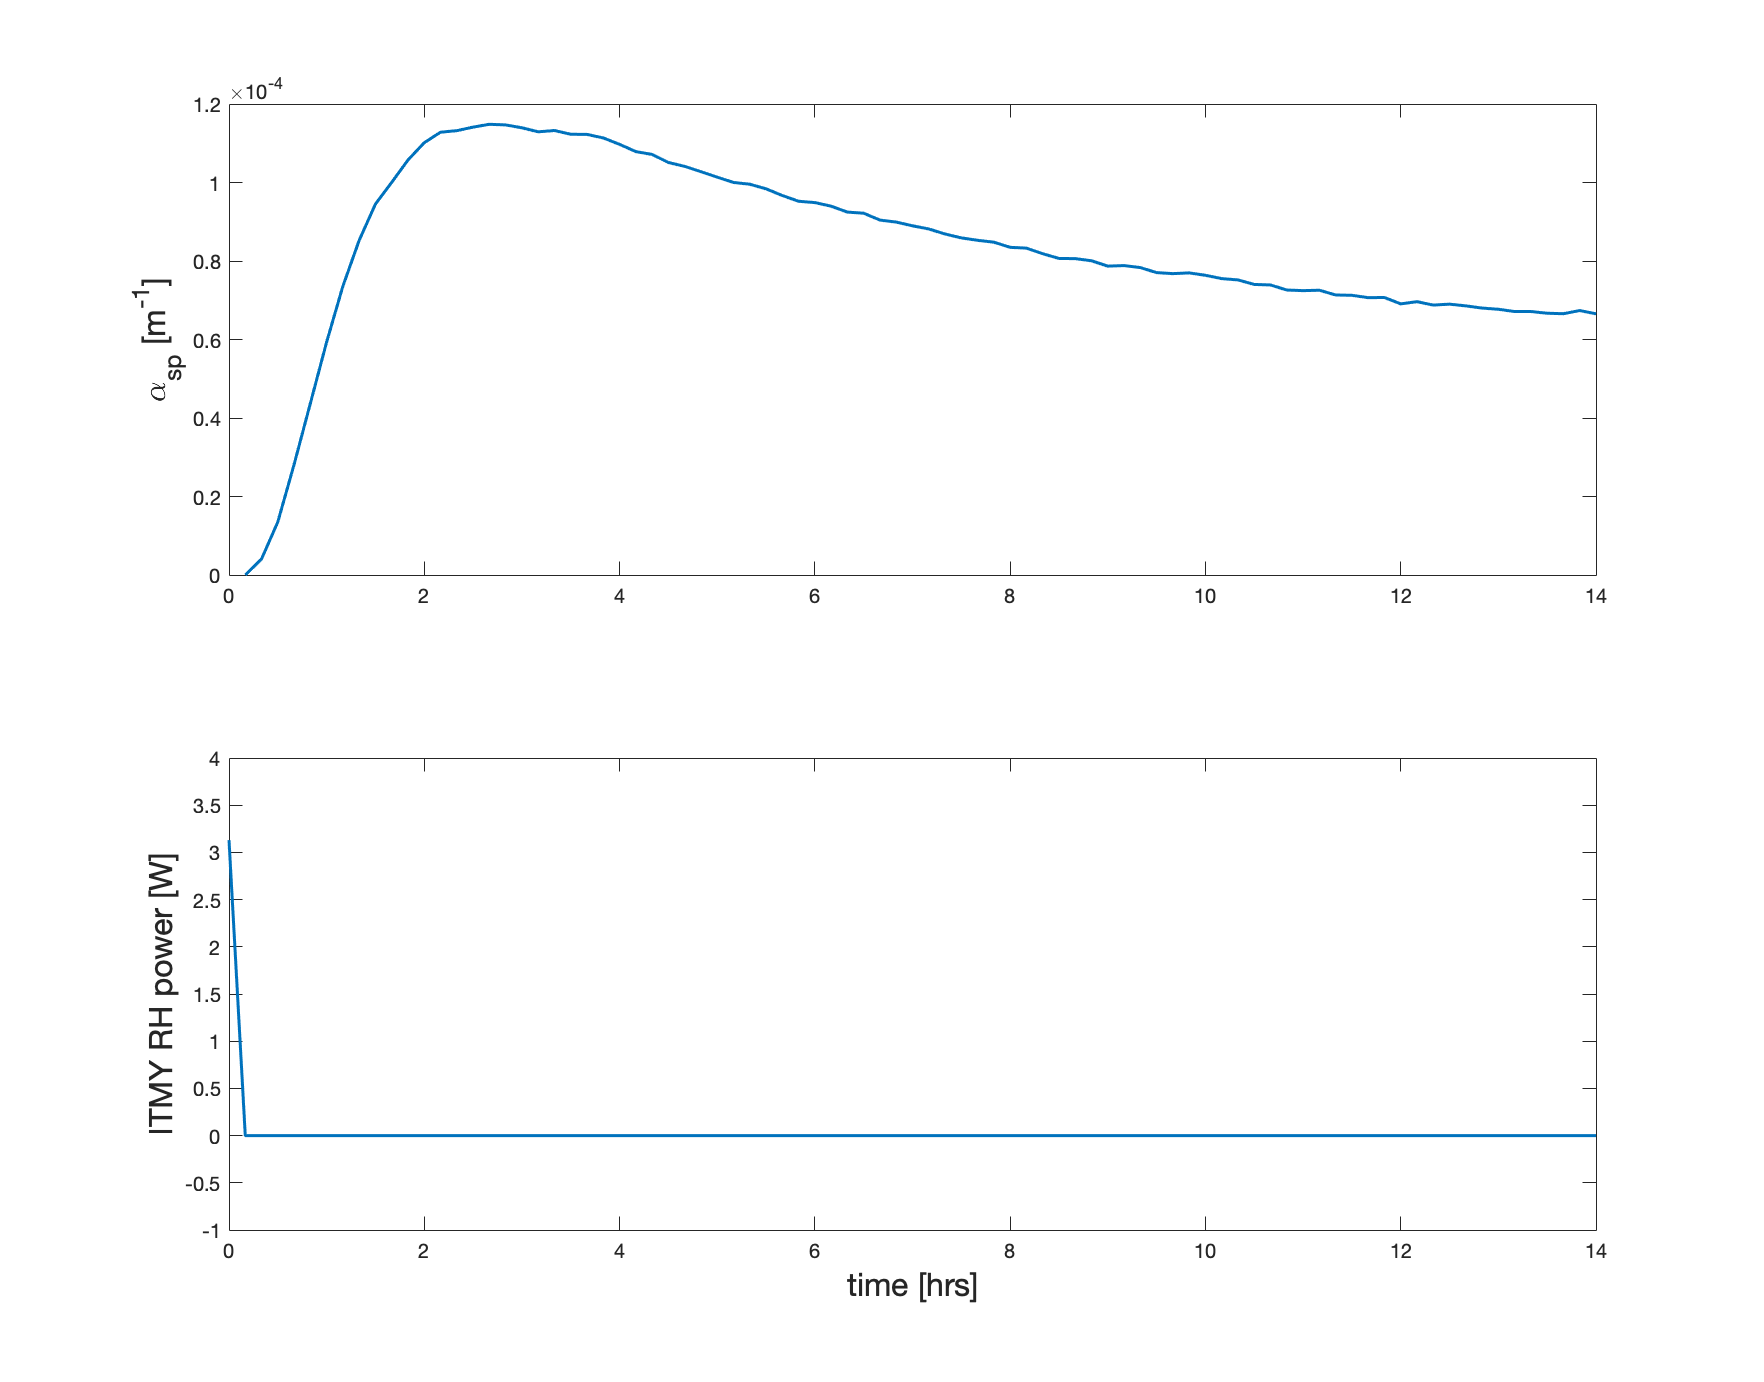
\includegraphics[width=\textwidth]{figures/matlab/ITMY_RH_power_step_decrease_measure.png}
 \caption{ITMY thermo-optic response to a 3.13 Watt power reduction to ring heaters. It's after $\approx$ 12 hours after the change was made do you start to see a small enough $\frac{\mathrm{d} \alpha_\mathrm{sp}}{\mathrm{dt}}$ when you can assume a steady thermal lens.}
 \label{fig:meas}
\end{figure}
%%%%%%%%%%%%%%%%%%%%%%%%%%%%%%%%%%%%%%%%%%%%%%%%%%%%%%%%%%%%%%%%%%%%%
%\newpage
\section{Concept}
\label{sec:III}

Before this method was implemented at the LIGO Hanford and Livingston sites, ring heater settings were adjusted by stepping the ring heater to a desired power though the thermo-optic step response function (H(s)) of the RH on ITMY (Fig [\ref{fig:meas}]) shows that for an approximate 10 hour period after your RH input power is changed,  $\frac{\mathrm{d}\alpha_{\mathrm{sp}}}{\mathrm{dt}}$ is nonzero. This long response time can be attributed to undermanaged heat being injected through the optic by stepping the power to the RH actuators.

\begin{figure}[H]
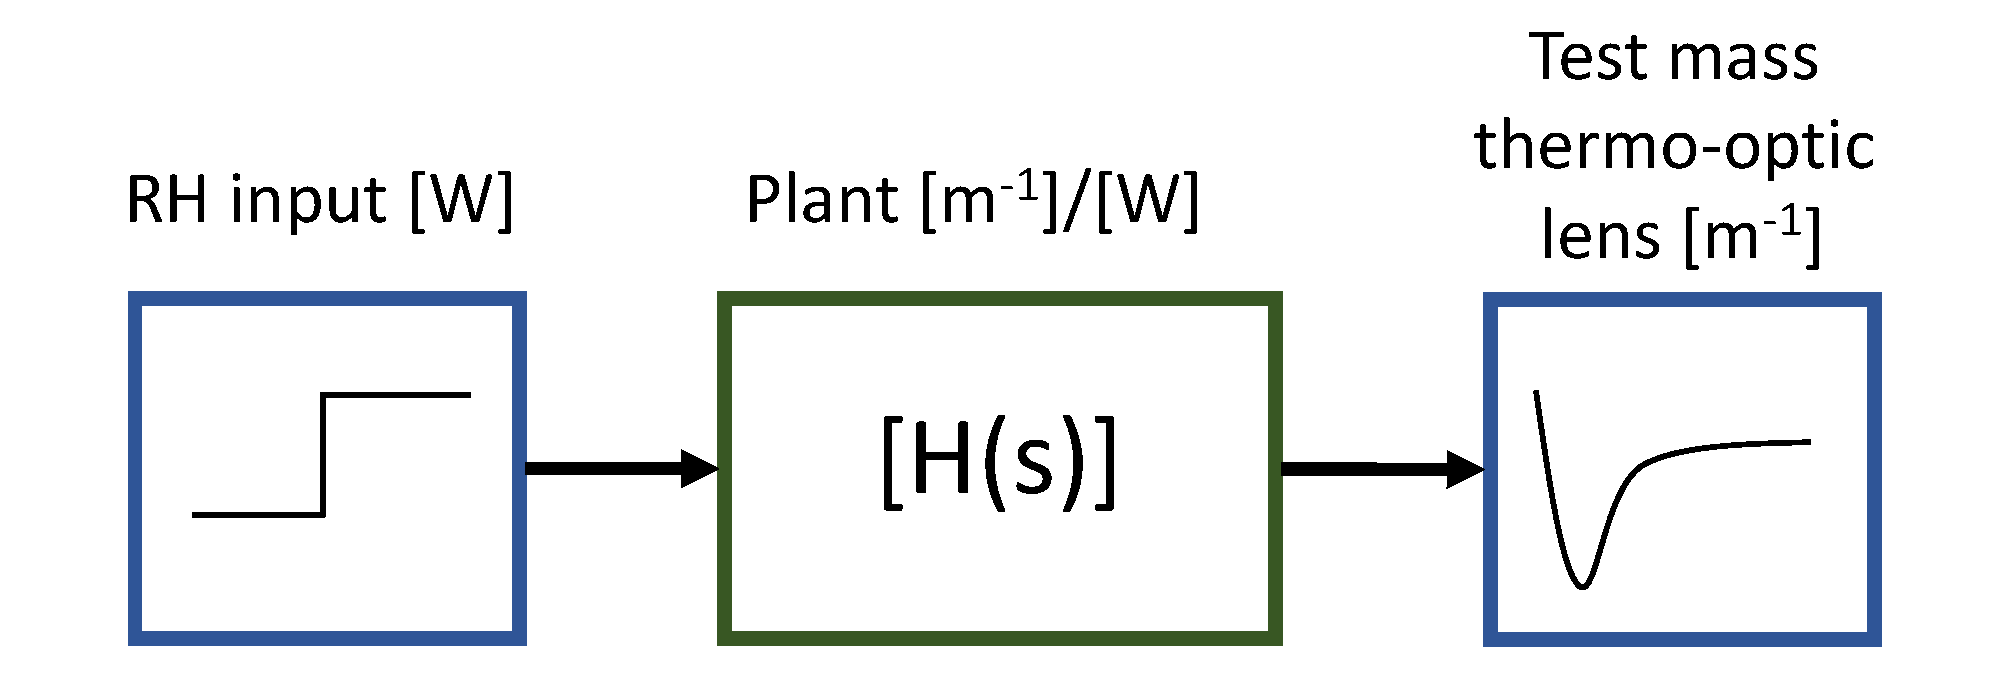
\includegraphics[page=1,width=\textwidth]{figures/RH_input_filter_figures.pdf}
\caption{A pictograph showing how the plant transforms the signal. The example of this can be seen in Fig [\ref{fig:meas}]}
\label{fig:justplant}
\end{figure}

For the most optimal management of injected RH power to the optic over time, constructing a real time digital filter custom made from the plant model (H(s)) will be critical to increasing the convergence speed of the RH/optic response. The first component to constructing this input RH filter ($[\mathrm{H}(\mathrm{s})]^{-1*}$) is inverting the ring heater thermo-optic step response. As will be seen in the next section, this suggests an unstable filter which motivates us to modify the inverse plant filter hence the asterisk in $[\mathrm{H}(\mathrm{s})]^{-1*})$.

\begin{figure}[H]
\includegraphics[page=2,width=\textwidth]{figures/RH_input_filter_figures.pdf}
\caption{A pictograph showing the system with real time digital filtering for an improved thermo-optic response. The RH input filter is created by inverting the plant filter combine with a low pass and added poles to the zpk model to ensure stability. }
\label{fig:plantwfilt}
\end{figure}



\section{Initial Filter Design}
\subsection{Plant filter (H(s))}

The plant filter was acquired by transforming the computed impulse response from [\ref{fig:meas}] into the Laplace domain and hand fitting a zpk filter over it.

\begin{figure}[H]
\includegraphics[page=2,width=\textwidth]{figures/matlab/plant_filter.png}
\caption{A comparison between the plant filter acquired from the measured ITMY RH step response data and the hand fitted H(s).}
\label{fig:plantfilt}
\end{figure}

The fitted zpk filter for ITMY is a one zero / three pole filter:


$$ H(s) = 9.2545*10^{-12} \frac{(s+3.142*10^{-5})}{(s+ 8.168*10^{-5}) (s+0.0003142) (s+0.0005969)} $$


\subsection{Inverse Plant filter (H$^{-1}$(s))}
\begin{figure}[H]
\includegraphics[page=2,width=\textwidth]{figures/matlab/inv_plant_filter.png}
\caption{Inverted plant filter H$^{-1}$(s)}
\label{fig:inv_plant_filt}
\end{figure}

$$ H^{-1}(s) = \frac{1}{9.2545*10^{-12}} \frac{(s+ 8.168*10^{-5}) (s+0.0003142) (s+0.0005969)}{(s+3.142*10^{-5})} $$

By just inverting the filter we have constructed a filter with a logarithmic rise in gain after .1 mHz. Implementing this filter without further modification would lead to high frequency artifacts in your ring heater power time series, suggesting a non-optimal response. Further modification is needed.



\subsection{Ring Heater input filter (Real time digital filter) ($[H(s)]^{*-1}$)}
An important modification was made after inverting the filter: 2 poles were added at -.0007 Hz to the same level of gain at DC ($<10^{-6}$Hz). This limit to the filter is necessary to reassure stability at .1 mHz.

\begin{figure}[H]
\includegraphics[page=2,width=\textwidth]{figures/matlab/IRHF.png}
\caption{The final form of the input RH filter for the ITMY RH.}
\label{fig:inv_plant_filt_mod}
\end{figure}

$$ [H(s)]^{-1*} = \frac{(s+8.168*10^{-5}) (s+0.0003142) (s+0.0005969)}{(s+3.142*10^{-5}) (s+0.0006994)^2} $$


\newpage
\subsection{Testing}
\subsubsection{Expected Performance}

\begin{figure}[H]
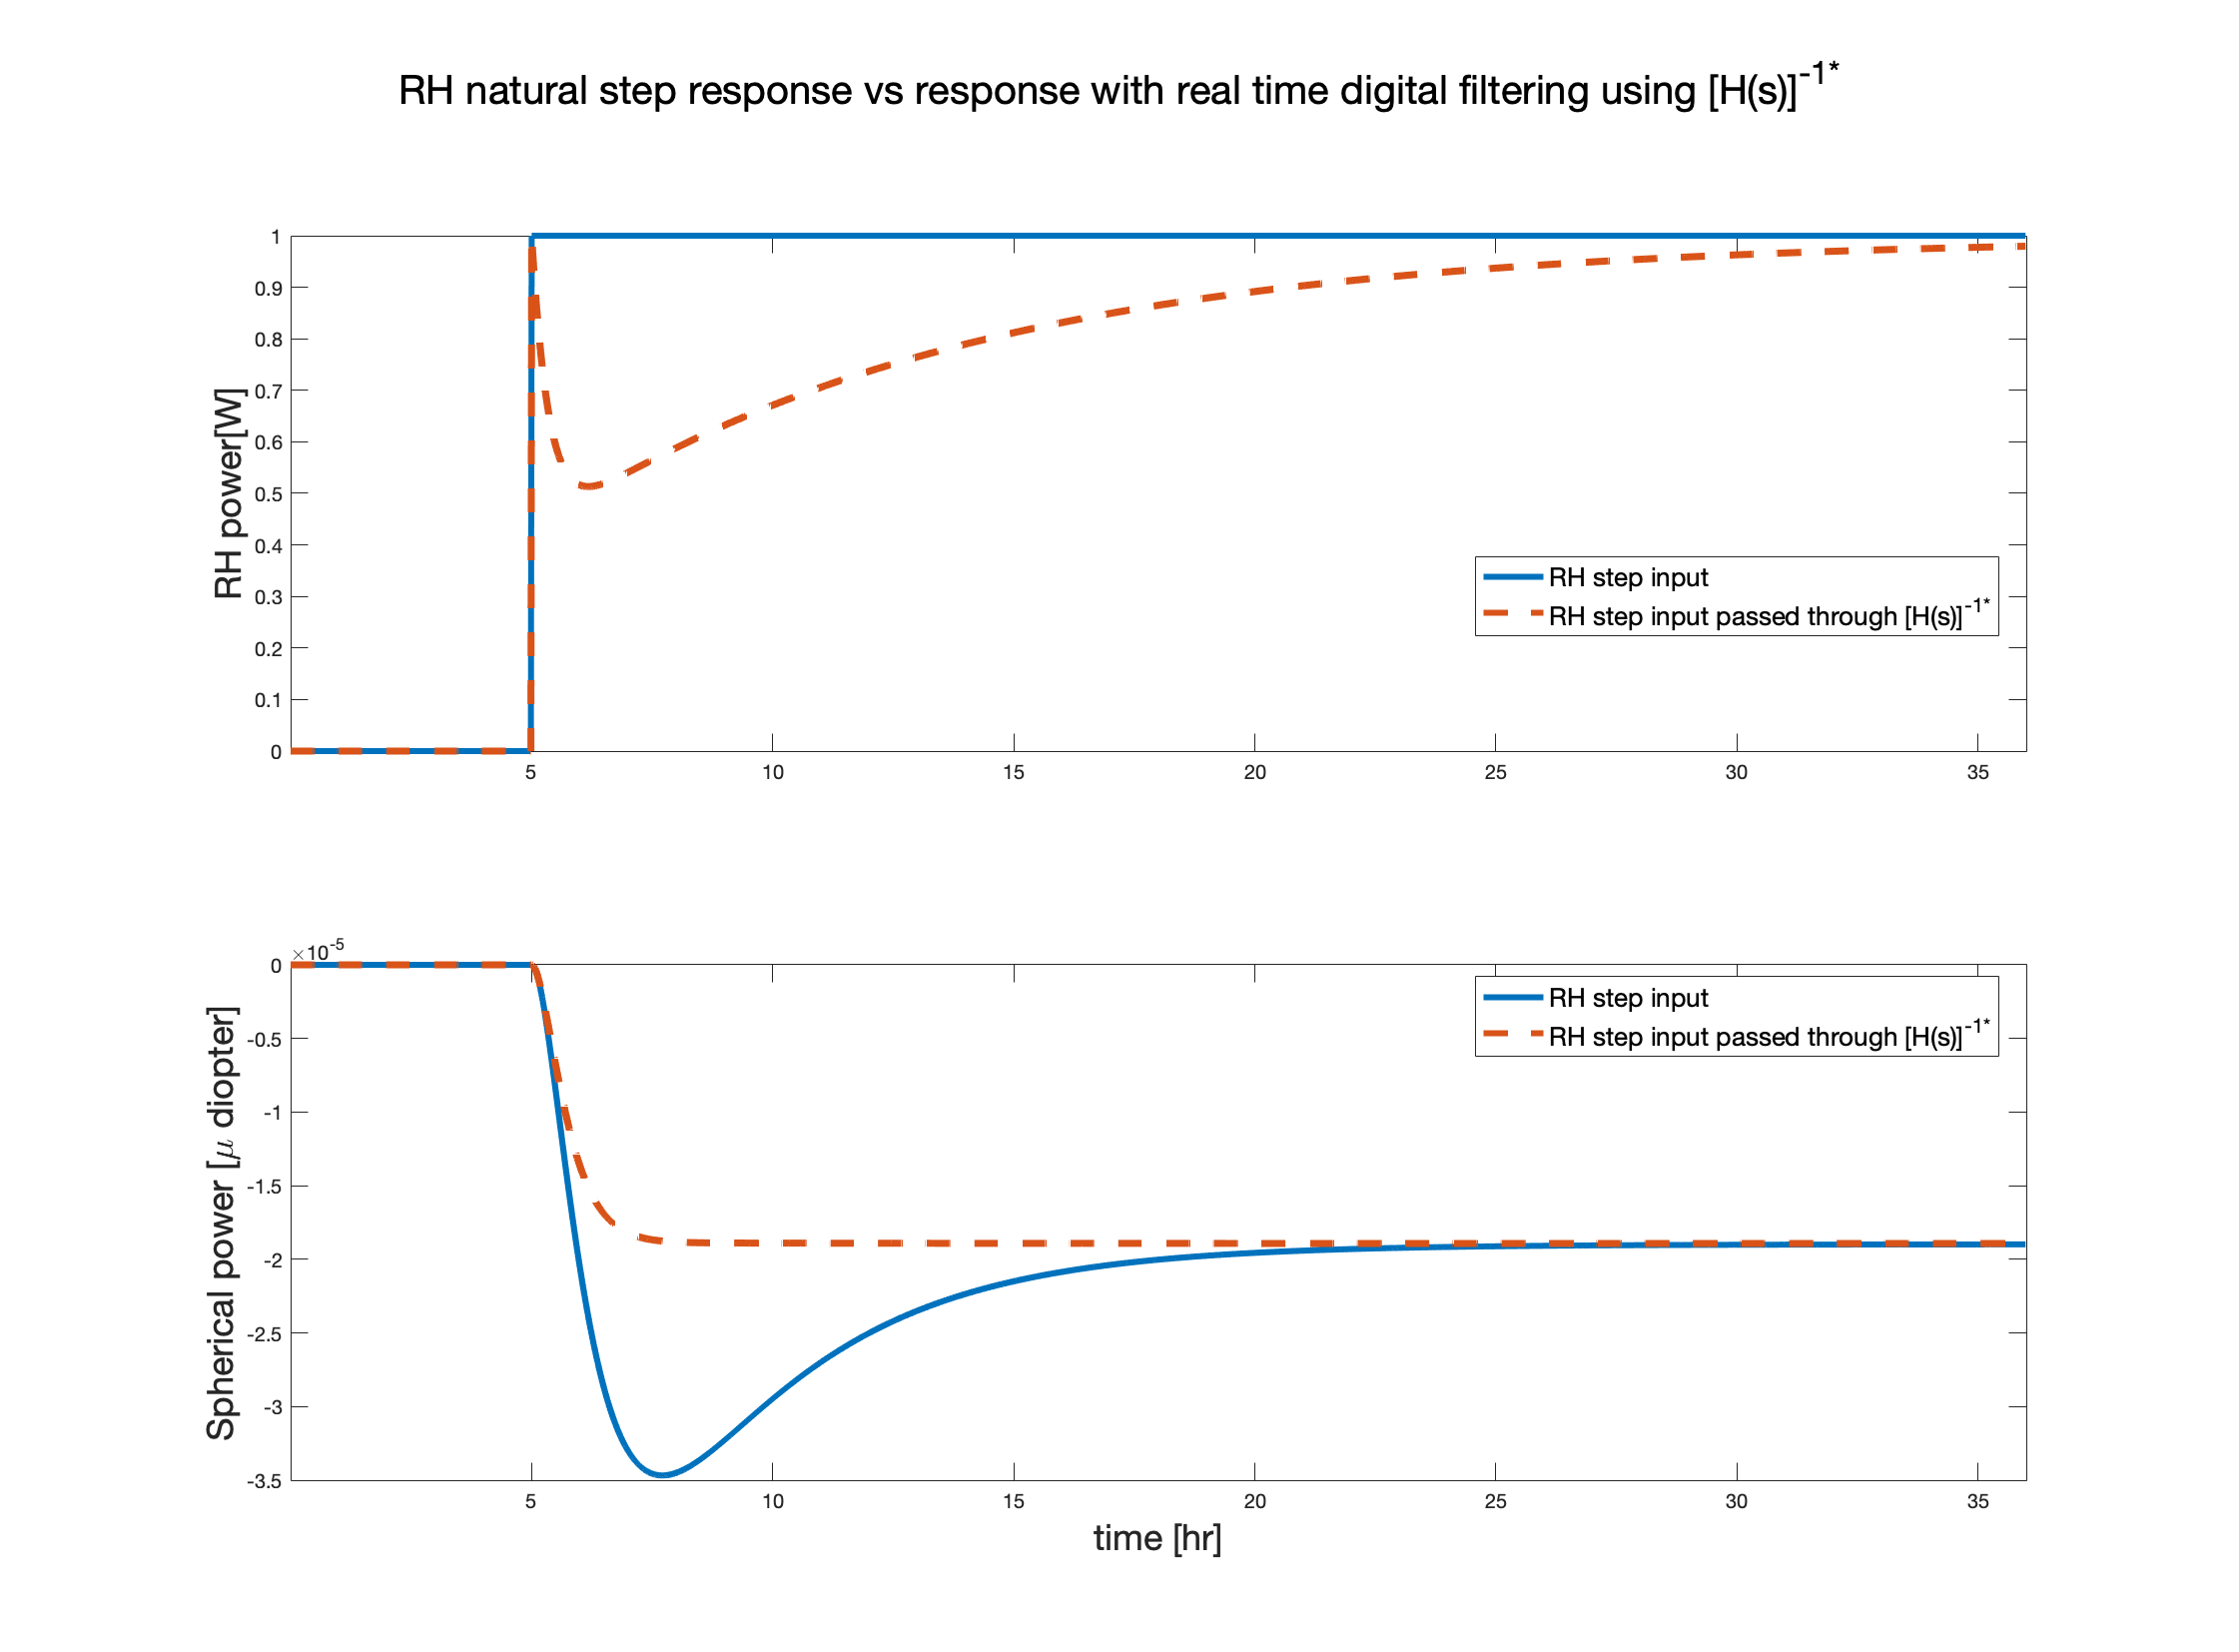
\includegraphics[width=\textwidth]{figures/matlab/PI_paper.png}
\caption{Comparison of the natural RH response and the response to the conditioned input. The above plot is simulated in Matlab by passing the RH input time series (top plot) through the $[H(s)]^{-1*}$ and $H(s)$ to acquire with the result lensing behavior on the bottom plot.}
\label{fig:comparison}
\end{figure}



\subsubsection{RH measurement at LHO}
Figure (?) demonstrates the performance of the filter for a ? W change of the RH at LHO:



\section{Extra considerations / Limitations}
Though the RH does reduce the mirror ROC convergence time by nearly a factor of 6, there needs to be discussion about the limitations of the filter. When inverting this filter we are demanding the most step-like thermo-optic response from our initial plant H(s). Therefore this could imply (look into this) that any more energy injected into the system would imply overshoot while any less would imply an undershoot. In a way the inversion suggests the most optimal time series.  This being said, we also must demand that the system remain stable in this chain of filters which requires that we limit the gain so that $[H(s)]^{-1*} \leq 1$ for $Re(s)/(2*\pi)>.1 \mathrm{mHz}$.

\section{Filter Modifications (for Dynamic Thermal Compensation)}
At LLO mitigating the ROC changes due to self heating is achieved through dynamic thermal compensation by adjustment of the RH actuators (at LHO it is achieved by reducing (central) CO2 heating) [refs]. If we use the above real time digital filtering we may soon realize that this is sub-optimal since $[H(s)]^{-1*}$ contains no information about self heating. Further filter design can be optimized by incorporating knowledge of the self heating response to the real time digital filter. \textcolor{red}{This can be done by generating an independent filter of the self heating response and multiplying it by $[H(s)]^{-1*}$. (Not sure if my brain did this right)}

This form of dynamic thermal compensation becomes crucial at high power (insert power mentioned in Terra's paper), not only to improve mode matching between coupled cavities but to avoid parametric instability (PI) [reference Terra's paper].


%%%%%%%%%%%%%%%%%%%%%%%%%%%%%%%%%%%%%%%%%%%%%%%%%%%%%%%%%%%%%%%%%%%%%

%\newpage

\begin{thebibliography}{99}


\end{thebibliography}

%%%%%%%%%%%%%%%%%%%%%%%%%%%%%%%%%%%%%%%%%%%%%%%%%
\newpage


\end{document}
